\intermediate{\subsection{Downloads and Installations}}

\step{Download and install \beast.}{
    \beast is available at
    \href{http://beast.bio.ed.ac.uk/Main_Page}{\url{http://beast.bio.ed.ac.uk/Main_Page}}.
    This tutorial is written for version 1.7.5 of \beast.
}

\step{Download data files from \todo{HERE}.}{
    All of the files needed for this exercise can be downloaded from \todo{HERE}.
    \begin{textbox}
        \centering
        \fbox{\begin{minipage}[c][8em][c]{0.5\textwidth}
            \ttfamily
            \begin{compactitem}
                \item div-time-tutorial/
                \begin{compactitem}
                    \item crocodylia-cytb.nex
                    \item div-time-tutorial.pdf
                    \item yule.py
                    \item output/
                    \begin{compactitem}
                        \item crocodylia-cytb-run1.log
                    \end{compactitem}
                \end{compactitem}
            \end{compactitem}
        \end{minipage}}
        \caption{The files required for this tutorial.}
    \end{textbox}
}

\intermediate{\subsection{Setting up XML file with \program{BEAUTi}}}

\step{Launch BEAUTi.}{Begin by launching the \program{BEAUTi} program. If you
    are using Mac OSX or Windows, you should be able to do this by double
    clicking on the application. If everything is working correctly, a window
    should appear that looks something like Figure~\ref{fig:beautiInit}.
    \begin{figure}[htbp]
        \centering
        \fbox{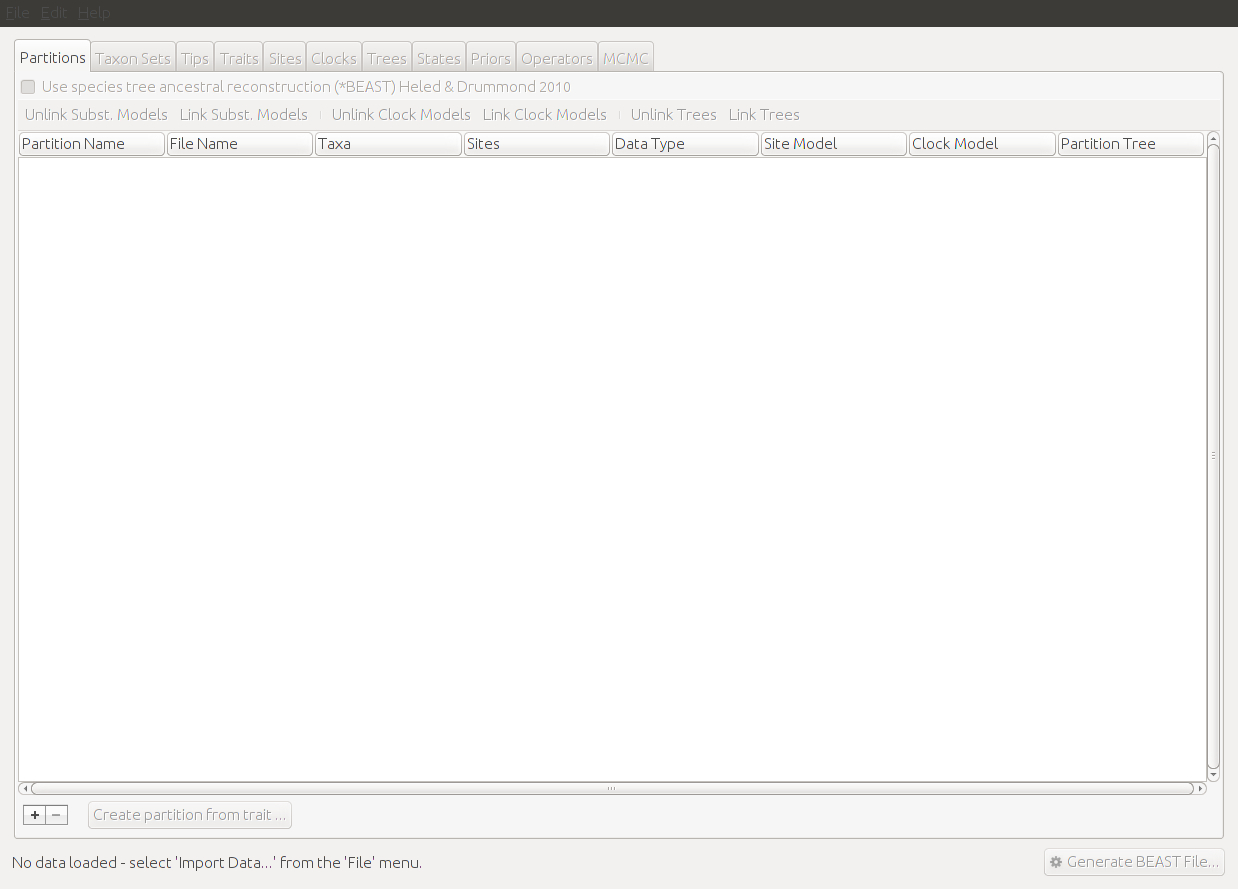
\includegraphics[width=0.7\textwidth]{../screenshots/beauti-init.jpg}}
        \caption{BEAUTi window.}
        \label{fig:beautiInit}
    \end{figure}
}

\step{Import the data in \localfile{crocodylia-cytb.nex}.}{
    Import the sequence data from the file \localfile{crocodylia-cytb.nex}
    using the drop-down menu \subItem{File}{Import Data} or using the
    \plusbutton button near the bottom-left corner of the window.

    You should be able to confirm that \program{BEAUTi} successfully imported
    24 sequences of nucleotides of length 1137
    (Figure~\ref{fig:beautiDataImported}).
    \begin{figure}[htbp]
        \centering
        \fbox{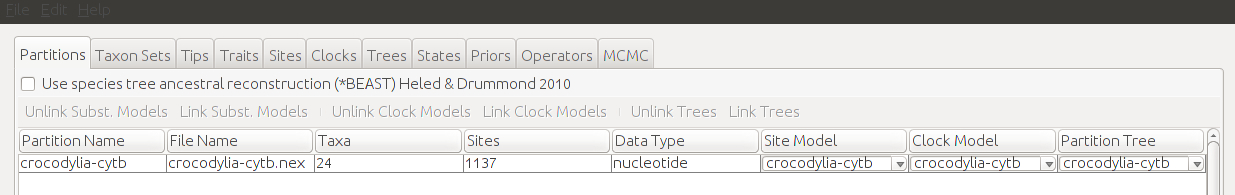
\includegraphics[width=0.8\textwidth]{../screenshots/beauti-data-imported.jpg}}
        \caption{The data successfully loaded by BEAUTi.}
        \label{fig:beautiDataImported}
    \end{figure}
}

\step{Inspect the alignment.}{
    Double click on the file name \localfile{crocodylia-cytb.nex} to bring up a
    window displaying the aligned sequences. It is always good practice to make
    sure everything looks as you expect. The cytochrome b gene is
    protein-coding, and aligns well across Crododylia without gaps.
}

\step{Define taxon sets.}{
    Next, we need to define some sets of taxa. Later, we will be able to use
    each of these sets to place priors on the age of their most recent common
    ancestor (MRCA).
    Let's start by defining the set for the clade
    containing the fossil taxon \emph{Navajosuchus mooki}; this clade has
    the family name Alligatoridae.

    Click on the \menutab{Taxon Sets} tab. Once in the \menutab{Taxon Sets}
    tab, click on the \plusbutton near the bottom-left corner of the window.
    This will create an untitled taxon set in the left-most box in the window.
    Change the name of this taxon set to \taxonset{Alligatoridae} and enter 65
    into Age column. This age is simply a starting value for the age of the
    MRCA of \taxonset{Alligatoridae}. It will ensure that the initial tree used
    to start the analysis is consistent with the lower bound of our fossil
    calibration (which will by 64 million years).
    
    We do not want to constrain \taxonset{Alligatoridae} to be monophyletic, so
    leave the \field{Mono?} box unchecked. Also, we are confident that
    \emph{Navajosuchus mooki} is nested within \taxonset{Alligatoridae}, and so
    we will leave the \field{Stem?} box unchecked. Because we only have a
    single tree, you can leave the \field{Tree} column unchanged.

    Next, we need to highlight the species that belong to
    \taxonset{Alligatoridae} within the \field{Excluded Taxa} window, and move
    them over to the \field{Included Taxa} window using the ``$\to$'' button.
    \taxonset{Alligatoridae} includes the following genera:
    \begin{compactitem}
        \item \emph{Alligator}
        \item \emph{Caiman}
        \item \emph{Melanosuchus}
        \item \emph{Paleosuchus}
    \end{compactitem}
    Highlight the species for these genera and move them over to the
    \field{Included Taxa} window.
    If you did everything correctly, your BEAUTi window should look like
    Figure~\ref{fig:beautiAlligatoridae}.
    \begin{figure}[htbp]
        \centering
        \fbox{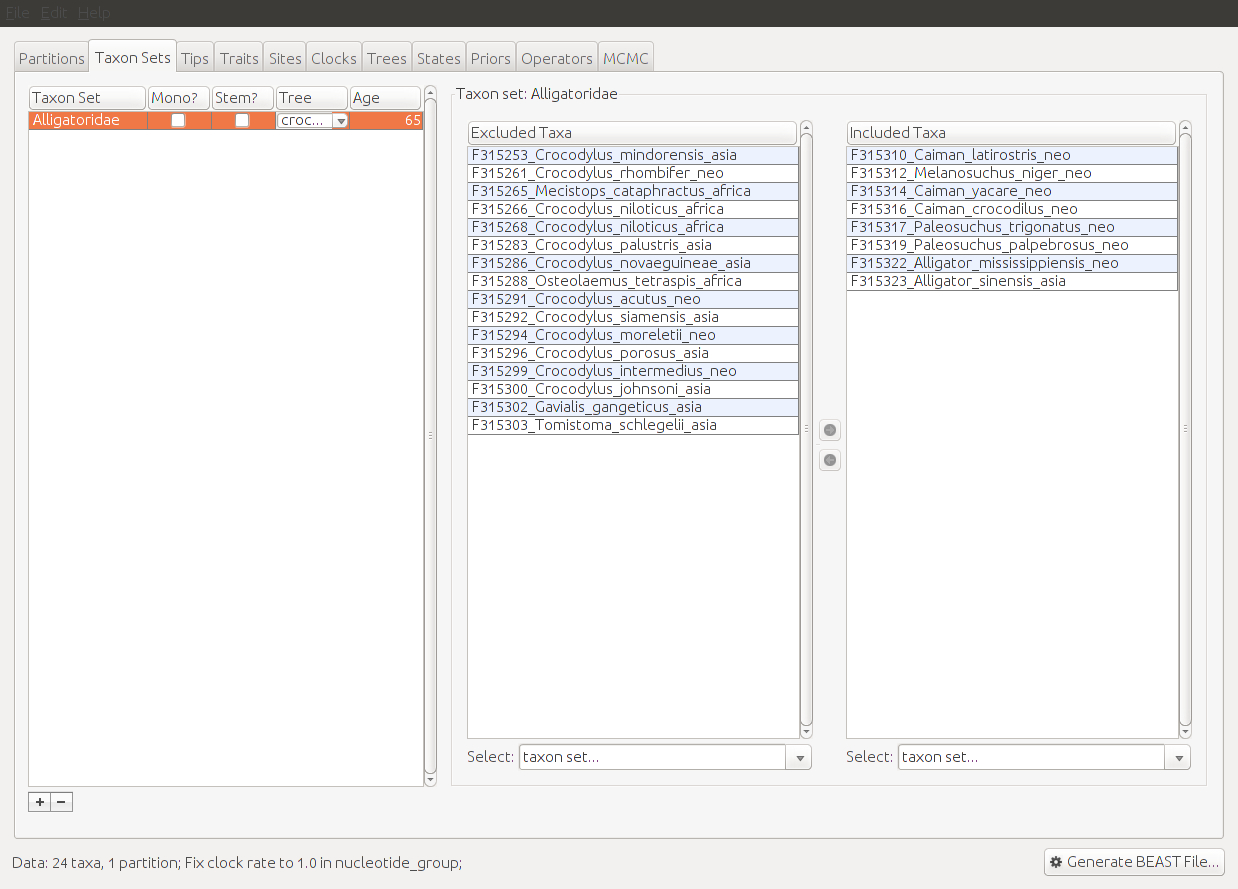
\includegraphics[width=0.9\textwidth]{../screenshots/beauti-taxon-set-alligatoridae.jpg}}
        \caption{The taxon set \taxonset{Alligatoridae} correctly defined.}
        \label{fig:beautiAlligatoridae}
    \end{figure}

    Next, let's define a taxon set for the genus \emph{Crocodylus}, which
    we will later use to specify an age prior corresponding to the fossil
    \emph{Crocodylus palaeindicus}. Click on the \plusbutton again to
    create a new taxon set, and name it \taxonset{Crocodylus}. Specify
    a starting age of 13, and leave the \field{Mono?} unchecked.

    We are confident that \emph{Crocodylus palaeindicus} is more closely
    related to all \emph{Crocodylus} species than to any other crocodylians.
    However, we are not confident that it is nested within extant species of
    \emph{Crocodylus} and suspect it is actually sister to them (as illustrated
    in Figure~\ref{fig:crocFossils}). As a result, we want to check the
    \field{Stem?} box. This specifies that the node we are interested in
    calibrating is the MRCA of all \emph{Crocodylus} sequences and their next
    closest relative (i.e., the stem node of \emph{Crocodylus}.
    Make sure the \taxonset{Crocodylus} taxon set is highlighted, and then
    highlight all the \emph{Crocodylus} species in the \field{Excluded Taxa}
    window and move them over to the \field{Included Taxa} window.

    Lastly, we need to define a taxon set for the genus \emph{Caiman}, which
    we will later use when specifying a calibration informed by the
    age of the oldest known \emph{Caiman} fossils.
    Click the \plusbutton to create a new taxon set, name it \taxonset{Caiman},
    specify a starting age of 10, and leave \field{Mono?} unchecked.
    As with \emph{Crocodylus} we don't know if the oldest \emph{Caiman} fossil
    taxa are nested within or sister to extant \emph{Caiman} species, and so
    we need to check the \field{Stem?} box.
    Highlight the three \emph{Caiman} species and move them over to the
    \field{Included Taxa} window.

    We will also be specifying a prior for the age of the root node of the
    tree, but we do not need to define a taxon set for this, because the root
    node is always defined by BEAUTi (you will see this later).

    Before you proceed to the next step, double check the three taxon sets
    you just defined and make sure you did not make a mistake with their
    ages or in selecting the species associated with them. Even a single
    misplaced species can lead to some very bizarre results!

    If you did everything correctly, your BEAUTi window should look similar to
    Figure~\ref{fig:beautiTaxSets}.

    \begin{figure}[htbp]
        \centering
        \fbox{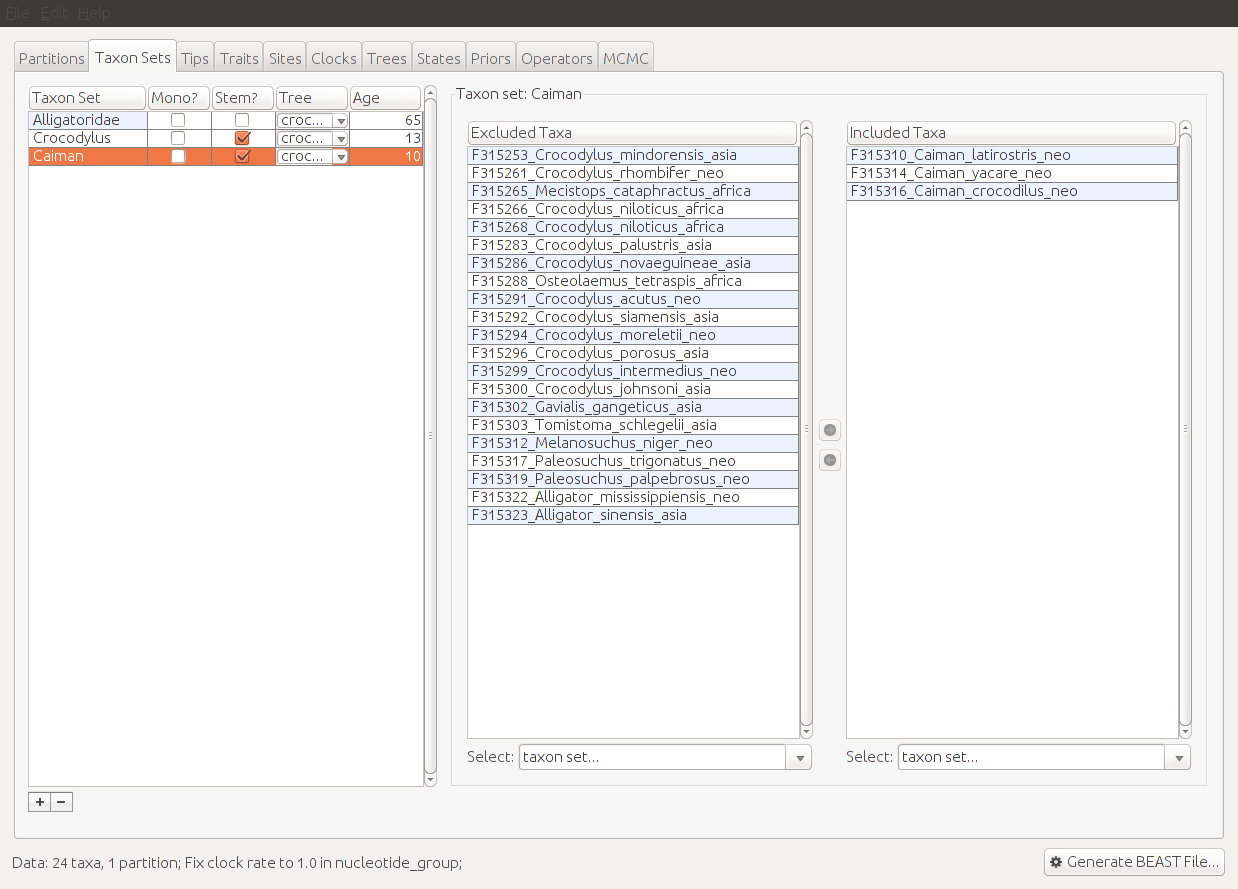
\includegraphics[width=0.9\textwidth]{../screenshots/beauti-taxon-sets.jpg}}
        \caption{All three taxon sets defined.}
        \label{fig:beautiTaxSets}
    \end{figure}
}

\step{Define geographic traits.}{
    Next we will use the \menutab{Traits} tab to define a new character for
    the geographic location of each species.
    This step is unrelated to divergence-time estimation. It will allow us to
    estimate the geographic locations of ancestral species across the
    phylogeny.
    Investigators are often interested in estimating ancestral states for
    characters of interest, so it is worth seeing how that can be done for in
    \beast while jointly estimating the phylogeny and divergence times.
    However, you will be learning all about ancestral character-state
    estimation in coming weeks, and so we will gloss over a lot of details to
    maintain the focus on divergence-time estimation.

    Once in the \menutab{Traits} tab, click the \plusbutton button (or the
    \field{Add trait} button). Once the \field{Create or Import Trait(s)}
    sub-window pops up, change the \field{Name} to \fieldvalue{geography}, set
    the \field{Type} to \fieldvalue{discrete}, and check the \field{Create a
    corresponding data partition} box
    (Figure~\ref{fig:beautiCreateTraitSubWindow}). Then, click \field{OK}.

    \begin{figure}[htbp]
        \centering
        \fbox{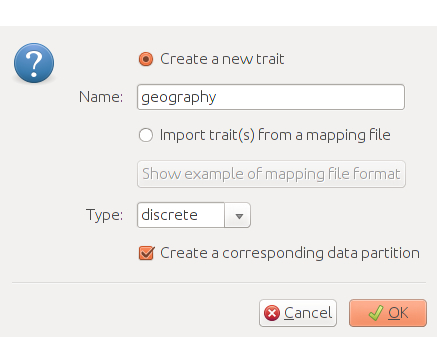
\includegraphics[width=0.4\textwidth]{../screenshots/beauti-create-trait-subwindow.jpg}}
        \caption{All three taxon sets defined.}
        \label{fig:beautiCreateTraitSubWindow}
    \end{figure}

    Next, click the \field{Guess trait values} button.  Once the sub-window
    pops up, select \field{Defined by its order} and set its drop-down field to
    \fieldvalue{last}. Put \fieldvalue{\_} (underscore) in the \field{with
    delimiter} field (Figure~\ref{fig:beautiGuessTraitSubWindow}). Click
    \field{OK}.
    If successful, the \menutab{Traits} tab should look like
    Figure~\ref{fig:beautiTraits}.

    \begin{figure}[htbp]
        \centering
        \fbox{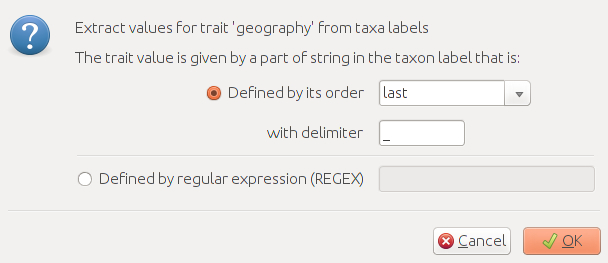
\includegraphics[width=0.5\textwidth]{../screenshots/beauti-guess-trait-subwindow.jpg}}
        \caption{All three taxon sets defined.}
        \label{fig:beautiGuessTraitSubWindow}
    \end{figure}

    \begin{figure}[htbp]
        \centering
        \fbox{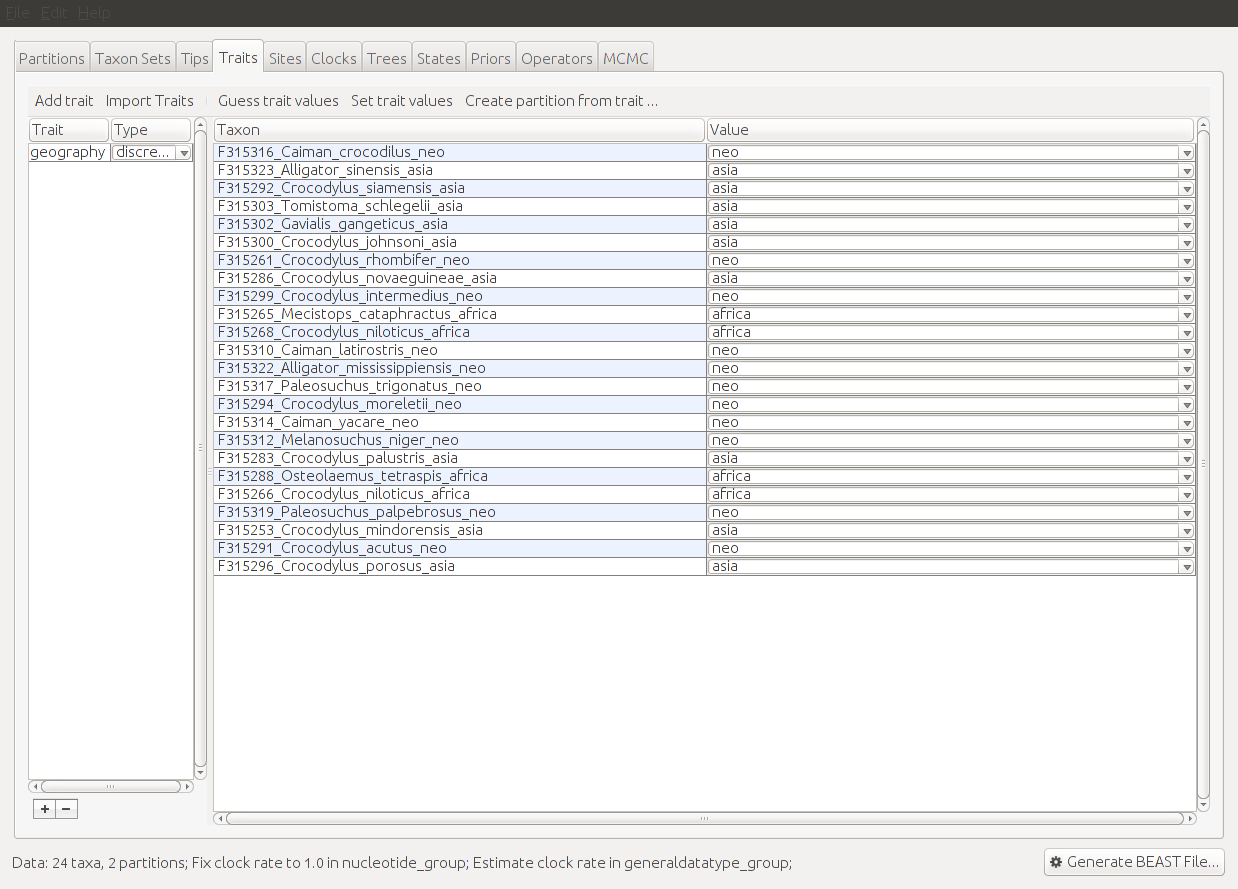
\includegraphics[width=0.8\textwidth]{../screenshots/beauti-traits.jpg}}
        \caption{All three taxon sets defined.}
        \label{fig:beautiTraits}
    \end{figure}
}

